%%%%%%%%%%%%%%%%%%%%%%%%%%%%%%%%%%%%%%%%%%%%%%%%%%%%%%%%%%%%%%%%%%%%%%%%%%%%%%%%
%%%%%%%%%% Author: Theo Park
%%%%%%%%%%%%%%%%%%%%%%%%%%%%%%%%%%%%%%%%%%%%%%%%%%%%%%%%%%%%%%%%%%%%%%%%%%%%%%%%
\documentclass{report}
\usepackage[utf8]{inputenc}

\usepackage{hyperref} % hyperlink for toc
\usepackage{palatino} % font
\usepackage{tikz}[matrix, backgrounds] % you know what tikz is

% Pkg used for both header and footer
\usepackage{fancyhdr}
% Header
\topmargin=-0.45in
\evensidemargin=0in
\oddsidemargin=0in
\textwidth=6.5in
\textheight=9.0in
\headsep=0.25in

\renewcommand{\footrulewidth}{0.4pt}

% Footer
\rfoot{\small{\textit{By Theo Park, based on Purdue Fall 2022 CS251}}}


\title{DSA Mini Textbook}
\author{Theo Park}
\date{}

\begin{document}

\maketitle

\pagestyle{fancy}

\tableofcontents

\chapter*{Preface}
\addcontentsline{toc}{chapter}{Preface}

% Chapter 1

\chapter{Runtime Analysis}

\textit{Algorithms} are any well-defined computational procedures that take some value(s) as input and produce more value(s) as output. They are \textbf{effective}, \textbf{precise}, and \textbf{finite}. There are several ways to analyze the runtime of an algorithm.

\section{Power Law}

\begin{enumerate}
  \item For the algorithm, get a table for the input size $n$ and the runtime $T(n)$.
    \begin{center}
      \begin{tabular}{ | c | c | } % c for center, l for left-align
        \hline
        $n$ & $T(n)$ \\
        \hline
        250 & 0.0 \\
        500 & 0.012 \\
        1000 & 0.0954 \\
        2000 & 0.7727 \\
        4000 & 6.1664 \\
        \hline
      \end{tabular}
    \end{center}
  \item Make sure that the data plots:
    \begin{itemize}
      \item \textbf{have enough data plots.} For instance, if there are only two data plots, you should not make the power law conjecture.
      \item \textbf{fits the power law.} You can verify this by finding the ratio between data plots.
        \begin{center}
          \begin{tabular}{ | c | c | c | }
            \hline
            $n$ & $T(n)$ & ratio \\
            \hline
            250 & 0.0 & -- \\
            500 & 0.012 & -- \\
            1000 & 0.0954 & 0.0954 / 0.012 = 7.95 \\
            2000 & 0.7727 & 0.7727 / 0.0954 = 8.10 \\
            4000 & 6.1664 & 6.1664 / 0.7727 = 7.98 \\
            \hline
          \end{tabular}
        \end{center}
    \end{itemize}
    For the ratios we found, 
\end{enumerate}

\section{Runtime Expressions}

\section{Asymptotic Runtime Analysis}

\section{Recursive Relationship}

% Chapter 2

\chapter{Intro to Data Structures}

\textit{Data structures} are collections of data values, the relationships among them, and the functions or operations that can be applied to the data. All three characteristics need to be present.

\section{Array}

\textit{Array} is a linear container of items.

\begin{center}
  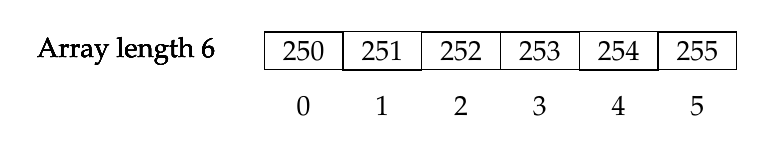
\begin{tikzpicture}
    \foreach \x in {0,...,5} {
      \node [left] at (-1,1) {Array length 6};
      \node [draw, minimum width=1cm] at (\x, 1) {25\x};
      \node at (\x, 0.3) {\x};
    } % foreach
  \end{tikzpicture}
\end{center}

\begin{itemize}
  \item Access time: $\Theta (1)$
  \item Inserting $n$ items in the \textit{tail} for array size $n$: $\Theta(1)$ per item, $n \times \Theta(1) \in \Theta(1)$
  \item Inserting $n$ items in the \textit{tail} for array size \textit{unknown}: $\Theta(n)$ per item, $n \times \Theta(n) \in \Theta(n)$
\end{itemize}

Lesson? \textbf{Keep track of the tail!}

\section{Linked List}

\section{Stack}

\section{Queue}

\section{Binary Heap}

\section{Tree}

% Chapter 3

\chapter{Sorting Algorithms}

\section{Bubble Sort}

\section{Selection Sort}

\section{Insertion Sort}

\section{Shell Sort}

\section{Heap Sort}

\subsection{Building a Heap -- Top-down v.s. Bottom-up}

\subsection{Sort Down Algorithm}

\section{Merge Sort}

\subsection{Merge Algorithm}

\section{Quick Sort}

\subsection{Pivot and Partition}

\section{Decision Tree and $\Omega{(n \log{n})}$ Limit for Comparison Sorting Algorithms}

\section{Counting Sort}

\section{Radix Sort}

% Chapter 4

\chapter{Hash Tables}

\section{Division Method}

\section{Multiplication Method}

\section{Collision}

\subsection{Chaining}

\subsection{Open Addressing}

% Chapter 5

\chapter{Search Tree}

\section{Binary Search Tree and Its Limit}

\section{2-3 Tree}

\section{Red-Black Tree}

\section{Left-Leaning Red-Black Tree}

\subsection{Deletion in LLRBT}

% Chapter 6

\chapter{Graph Traversal}

\section{Adjacency Matrix and List}

\section{DFS}

\section{BFS}

% Chapter 7

\chapter{Directed Graphs}

\section{Strong Connectivity}

\subsection{Brute-force Strong Connectivity Algorithm}

\subsection{Brute-force using Stack}

\subsection{Strongly Connected Components and Kosaraju's Algorithm}

\section{Directed Acyclic Graphs}

\subsection{Topological Sort}

% Chapter 8

\chapter{Weighted Graphs}

\section{Shortest Path}

\subsection{Dijkstra's Algorithm}

\subsection{Bellman-Ford Algorithm}

\section{Articulation Points}

\section{Minimum Spanning Tree}

\subsection{Cycle and Cut Properties}

\subsection{Prim's Algorithm}

\section{Union-Find}

\subsection{Kruskal MST Algorithm}

% Chapter 9

\chapter{Strings}

\section{Brute-force String Pattern Matching}

\section{KMP Algorithm}

\section{Trie}

\section{PATRICIA}

\section{Huffman Coding}

\end{document}
